	\documentclass[a4paper,titlepage]{article}
	\usepackage[utf8]{inputenc}
	\usepackage[export]{adjustbox}
	\usepackage[french]{babel}
	\usepackage{hyperref}
	\usepackage{graphicx}
	\usepackage{fourier}
	\usepackage{color}   %May be necessary if you want to color links
	\usepackage{hyperref}
	\definecolor{GreyBlack}{RGB}{92, 89, 92}
	\hypersetup{
    		colorlinks=true, %set true if you want colored links
    		citecolor=black,
    		citecolor=black,
    		filecolor=black,
   			linkcolor=GreyBlack,
    		urlcolor=magenta
    }
	\usepackage[margin=1.3in]{geometry}
	\author{Baptiste Vergote & Martin Schreinemachers}
	\begin{document}
	% Page de titre
	\titlepage{
		16 Décembre 2014 \\[2cm]
		\begin{center}\sf\Huge
		{\bfseries \underline{Document 3 :}} \\[2mm]
		{\bfseries Langage avancé de programmation} \\[1cm]
		\begin{figure}[!h]
		\centering
			\includegraphics[scale=0.55]{EcranCarte.png}
		\end{figure}
		\begin{center}
		{\huge RPG - The Epic School Adventure}
		
		\end{center}
		
		\end{center}
		\ \\[4cm]
		\textbf{Baptiste Vergote \& Martin Schreinemachers 2TL2} \\
		EPHEC LLN -- 2014-2015
	}
	\clearpage
	\tableofcontents
	\clearpage
	\section*{TODO}
	\begin{enumerate}
		\item Un document word comprenant : 
		\begin{enumerate}
			\item Une page de garde (noms, prénoms, class, titre du projet, un screenshot du projet, année académique).
			\item Une introduction où vous présentez votre projet.
			\item Le diagramme UML des classes OO que vous avez (ou un extrait intéressant).
			\item Un texte expliquant tout ce qui est nécessaire pour que votre projet fonctionne (modification du path, driver à installer et dans ce cas les fournir, …).
			\item Quelques screenshots de votre projet (idéalement pour illustrer des passages de votre travail – donc vous ne faites pas un titre screenshot mais vous en mettez là où c’est utile).
			\item Le code source (ou un extrait représentatif) documenté du package principal de l’application (+fichier package-info.java).
			\item La documentation du package principal (fichiers html générés par la javadoc).
			\item Une description de votre stratégie de validation.
			\item Une conclusion : que vous a apporté ce projet, quelles ont été les difficultés rencontrées, comment peut-on l’améliorer.
		\end{enumerate}
		\item Tous vos codes sources et tests unitaires (le projet eclipse).
		\item Le fichier JAR de votre application.
	\end{enumerate}
	\clearpage
	\section{Introduction}
	\textit{Une introduction où vous présentez votre projet. -> A SUPPRIMER}\\
	
	Dans un petite bourgade en plein centre du monde que j'attire votre attention...\\
	Dans les environs de Louvain-La-Neuve, c'est en amont d'un lac puant que l'aventure a démarré...\\
	
	Une journée bien trop remplie... 3 heures à rester assis, à écouter et suivre, sans un mot ( ou ?de cours d'affilées), un challenge que peu arrive à endurer. C'est en êtres surhumains que les deux apprentis programmeurs, dont nous parlerons plus tard, se sont lancés dans un projet fou, insensé et sans fin..\\
	
	Actuellement, ils sommes assis dans une classe trop sombre, trop petite, qui sent la transpiration... Interdit/empécher(autre à trouver?) d'aérer à cause des autochtones qui peuplent l'établissement... Ceux ci ne cesse de l'empester de leurs parfums et de leurs fumées ragoutantes/répugnantes... Quel supplice de devoir les supporter au quotidien...\\
	Ces derniers sont prèts à tout pour bouter nos héros hors de leur forteresse(chateau/royaume(?)).\\
	
	Mais nos deux héros, accompagnés d'une poignée, sont des durs à cuire, ils subissent des attaques de toute part mais ne flanchent pas(tiennent bon? (non, suite<-))..\\ 
	Ils tiennent tête(s?) à ces soldats fous, fervants défenseurs des grands champions, "Ceux-dont-on-ne-doit-pas-prononcer-le-nom".\\
	
	Encourage par leurs proches, nos deux programmeurs aliénés/déséquilibrés(=Fou a l'extreme) se sont lancés dans l'aventure/expédition/odyssée/épreuve.\\
	Accompagné de leur PC et de leurs cerveaus, affaiblis par les attaques répétées, ils ont commencé à imaginer un moyen d'arriver(non, autre) à leur but ultime (NO SPOIL !!).\\
	
	Serez vous assez fort pour les aider?\\
	
	Parviendrez vous à arrêter toutes les menaces auxquels vous serez confrontés?\\
	Si oui, suivez nous, arpentez vous dans ces contrées dangereuse et devenez protecteur des faibles et des opprimés!
	
	\clearpage
	\section{Diagramme UML}
	Le diagramme UML des classes OO que vous avez (ou un extrait intéressant).\\
	\subsection{Package PPersonnage}	
	
	Dans ce package est compris tout ce qui constitue et gère les personnages
	\begin{figure}[h!]
		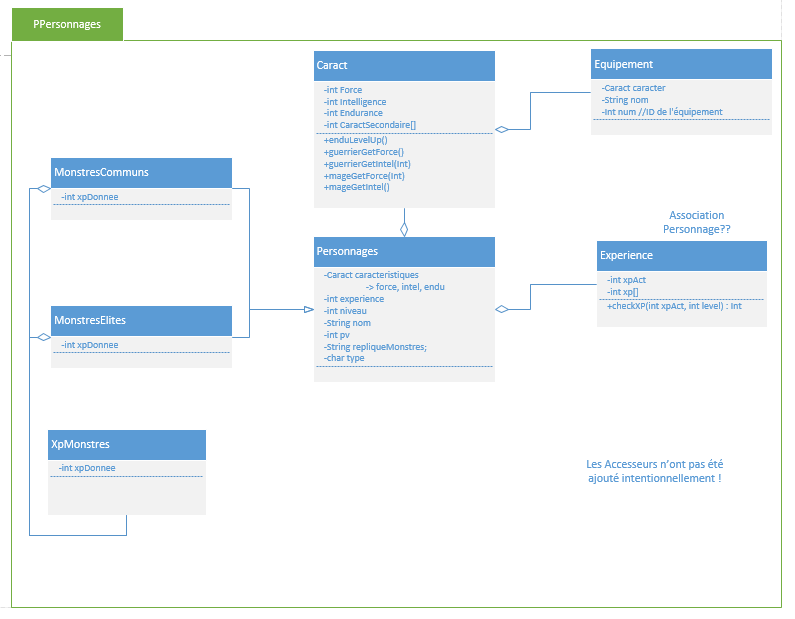
\includegraphics[scale=0.70]{PPersonnage.png}
	\end{figure}
	\clearpage
	
	\section{Necessité pour la fonctionnalité}
	Un texte expliquant tout ce qui est nécessaire pour que votre projet fonctionne (modification du path, driver à installer et dans ce cas les fournir, …).
	\clearpage
	
	\section{Notre jeu étapes par étapes}
	En double cliquant sur le fichier JAR, le jeu se lance en plein écran, vous laissant apercevoir un magnifique écran de démarrage :
	\begin{figure}[h!]
		\includegraphics[scale=0.30]{EcranDebut.jpg}
	\end{figure}
	
	Sur cette image, trois boutons sont présents : 
	\begin{enumerate}
		\item Le bouton de création d'une Nouvelle Partie.
		\item La bouton permettant de Continuer la partie en cours.
		\item Un bouton pour changer les options.
	\end{enumerate}
	
	En cliquant sur "Nouvelle Partie", un écran de sélection de personnage apparait :
	\begin{figure}[h!]
		\includegraphics[scale=0.30]{EcranCreationPersonnage.jpg}
	\end{figure}
	
	Vous cliquez sur le personnage que vous souhaitez jouer, lui entrez un Pseudo et le jeu commence :
	\begin{figure}[h!]
		\includegraphics[scale=0.65]{EcranCarte.png}
	\end{figure}
	
	Comme vous pouvez le constater, le guerrier apparait dans le coin supérieur gauche de la carte, celle-ci délimitée par les petits cailloux que vous ne pourriez, bien entendu, pas traverser ;) !\\
	
	En se baladant dans la prairie, celui ci va se heurter à des rencontres inattendues ou notre champion va devoir vendre chèrement sa peau !\\
	
	Nous ne dévoilerons pas la suite, à vous de la découvrir !\\
	
	Bonne chance dans cet univers rempli de monstres sanguinaires !
	\clearpage
	
	\section{Documentation du package}
	La documentation du package principal (fichiers html générés par la javadoc).
	\clearpage
	
	\section{Description de la stratégie de validation}
	Une description de votre stratégie de validation.
	\clearpage
	
	\section{Difficultés rencontrées}
	La première difficulté pour nous était d’appréhender le problème de conception de notre jeu. Quels éléments intégrer (monstres de différents types ? Leur permettre de sortir des répliques ? Implémenter un système d’équipements ?), comment les intégrer, comment séparer tout ces éléments logique en classes…\\
	
Rapidement suivi par nos débuts avec les interfaces graphiques. D’abord, nous sommes partis sur une interface plus simple utilisant les libraires swing, sur le conseil d’un camarade, nous nous sommes redirigés vers les librairies Slick2d qui facilitent grandement l’implémentation de jeu en 2D.\\

Pour Slick2d, la difficulté résidait d’abord dans le fait qu’on utilisait des classes écrites par d’autres et dont on ne voit pas toujours le code...\\ L’habitude venant avec la pratique, ce problème s’est rapidement résolu pour la plupart des cas. Vient ensuite une bêtise qui nous à fait perdre beaucoup de temps : Slick2d \og réinvente \fg{} Java. Pour indiquer un chemin vers une image, un fichier de musique, il faut commencer par le nom du dossier $/$ du fichier lui-même alors qu'habituellement, on indique le début d’un chemin par un \og $/$ \fg{}. \\

Autre perte de temps, les coordonnées des objets sont calculées à partir du coin inférieur gauche de l’écran, et non à partir du coin supérieur gauche...\\

Les classes que nous avons utilisés dans Slick2d nous ont permis de créer un jeu basé sur des états, ceux-ci déterminant chacun un écran et une étape de jeu.
	\section{Conclusion}
	Une conclusion : que vous a apporté ce projet, quelles ont été les difficultés rencontrées, comment peut-on l’améliorer.\\
	\\
	\\
	Martin adorait l'idée d'un RPG, étant tous les deux des joueurs de RPG, nous nous sommes lancés très vite dans l'idée.
	\clearpage
	\section*{Sources }
\danger Nous ne nous sommes pas préoccupés, dans le cadre de ce projet des éventuels droits d'auteurs.\\

Il est aussi important de préciser que les images ont été redimmensionné et parfois coupé pour les besoins de ce projet.	
	
\subsubsection*{Bibliographie :}

\begin{itemize}
	\item Les bibliothèques de l'université de Louvain-La-Neuve. (2013) \textit{Rédiger une bibliographie au format APA.} Lien du PDF sur : \url{http://www.uclouvain.be/cps/ucl/doc/bpsp/documents/Bibliographie\_APA\_F\_13doi.pdf},  consultée le 13 décembre 2014.
	\item Pharmacritique. (2009). \textit{Le rapport de l'IGAS donne une idée des conflits d'intérêts financiers des médecins travaillant pour l'industrie et des intérêts autres qui biaisent la recherche médicale.} En ligne sur \url{http://pharmacritique.20minutes-blogs.fr/archive/2009/02/07/le-rapport-de-l-igas-nous-donne-une-idee-des-conflits-d-inte.html}, consultée le 10 décembre 2014.
	\item La pub de tropicalboy. (2006). \textit{Royal Canin}. En ligne sur \url{http://mapubamoi.canalblog.com/archives/2006/04/13/1694142.html}, consultée le 10 décembre 2014.
	\item Le devoir, libre de penser. (2007). \textit{Les caricatures de Garnotte}. En ligne sur \url{http://www.ledevoir.com/galeries-photos/les-caricatures-de-garnotte/71304}, consultée le 10 décembre 2014.
	\item Les experts Denjean associés. (2014). \textit{Quiz : Quel professionnel comptable êtes-vous?} En ligne sur \url{http://www.les-experts-denjean-associes.com/test-quel-genre-dexpert-comptable-etes-vous/}, consultée le 10 décembre 2014.
	\item Funny Art Pictures. (2008). \textit{Ultimate Attraction.} En ligne sur \url{http://www.funnyartpictures.com/pics-funny-stuff/?images/midsize/signs-ads/ultimate-attraction.jpg}, consultée le 10 décembre 2014.
	\item GoPixPic. (Date inconnue). \textit{Games Returns In the Guild Wars 2...} En ligne sur \url{http://www.gopixpic.com/640/-games-returns-in-the-guild-wars-2-warrior-classes/http:||guides*gamepressure*com|guildwars2|gfx|word|978182984*jpg/}, consultée le 1 décembre 2014.
	\item Guild Wars 2 - Profession - Élémentaliste. (Date inconnue entre 2010 et 2014). \textit{Fond d'écran - Élémentaliste.} En ligne sur \url{https://www.guildwars2.com/fr/the-game/professions/elementalist/}
	\item Color picker with high precision and contrast test. (Date inconnue) \textit{Color picker.} En ligne sur \url{http://colorizer.org/}, consultée le 1 décembre 2014.
	\item OpenClassrooms. (Date inconnue). \textit{Apprenez à programmer en Java - Positionner des boutons.} En ligne sur \url{http://openclassrooms.com/courses/apprenez-a-programmer-en-java/positionner-des-
boutons}
	\item Wikipédia. (Dernière modification le 10 décambre 2014). \textit{Noms de couleur du Web.} En ligne sur \url{http://fr.wikipedia.org/wiki/Couleurs_du_Web}.
	\item Apprendre Java - Cours et exercices. (2011). \textit{Les interfaces graphiques en Java.} En ligne sur \url{http://www.infres.enst.fr/~hudry/coursJava/interSwing/index.html}
	\item Open Game Art. (Date inconnue) \textit{Morning Sunrise Background.} En ligne sur \url{http://opengameart.org/content/morning-sunrise-background}
	\item Shionn::blog() - Be a geek. (Date inconnue). \textit{Tutoriels slick 2D.} En ligne sur \url{http://www.shionn.org/tutoriels-slick-2d}
\end{itemize}
	
	\clearpage	
	\end{document}